%package list
\documentclass{article}
\usepackage[top=3cm, bottom=3cm, outer=3cm, inner=3cm]{geometry}
\usepackage{multicol}
\usepackage{graphicx}
\usepackage{url}
%\usepackage{cite}
\usepackage{hyperref}
\usepackage{array}
%\usepackage{multicol}
\newcolumntype{x}[1]{>{\centering\arraybackslash\hspace{0pt}}p{#1}}
\usepackage{natbib}
\usepackage{pdfpages}
\usepackage{multirow}
\usepackage[normalem]{ulem}
\useunder{\uline}{\ul}{}
\usepackage{svg}
\usepackage{xcolor}
\usepackage{listings}
\lstdefinestyle{ascii-tree}{
	literate={├}{|}1 {─}{--}1 {└}{+}1 
}
\lstset{basicstyle=\ttfamily,
	showstringspaces=false,
	commentstyle=\color{red},
	keywordstyle=\color{blue}
}
%\usepackage{booktabs}
\usepackage{caption}
\usepackage{subcaption}
\usepackage{float}
\usepackage{array}

\newcolumntype{M}[1]{>{\centering\arraybackslash}m{#1}}
\newcolumntype{N}{@{}m{0pt}@{}}


%%%%%%%%%%%%%%%%%%%%%%%%%%%%%%%%%%%%%%%%%%%%%%%%%%%%%%%%%%%%%%%%%%%%%%%%%%%%
%%%%%%%%%%%%%%%%%%%%%%%%%%%%%%%%%%%%%%%%%%%%%%%%%%%%%%%%%%%%%%%%%%%%%%%%%%%%
\newcommand{\itemEmail}{jchuraaca@unsa.edu.pe}
\newcommand{\itemStudent}{Julio Rubén Chura Acabana}
\newcommand{\itemCourse}{ F. de Programción 2}
\newcommand{\itemCourseCode}{20230472}
\newcommand{\itemSemester}{I}
\newcommand{\itemUniversity}{Universidad Nacional de San Agustín de Arequipa}
\newcommand{\itemFaculty}{Facultad de Ingeniería de Producción y Servicios}
\newcommand{\itemDepartment}{Departamento Académico de Ingeniería de Sistemas e Informática}
\newcommand{\itemSchool}{Escuela Profesional de Ingeniería de Sistemas}
\newcommand{\itemAcademic}{2023 - B}
\newcommand{\itemInput}{Del 11 Octubre 2023}
\newcommand{\itemOutput}{Al 16 Octubre 2023}
\newcommand{\itemPracticeNumber}{06}
\newcommand{\itemTheme}{ArrayList}
%%%%%%%%%%%%%%%%%%%%%%%%%%%%%%%%%%%%%%%%%%%%%%%%%%%%%%%%%%%%%%%%%%%%%%%%%%%%
%%%%%%%%%%%%%%%%%%%%%%%%%%%%%%%%%%%%%%%%%%%%%%%%%%%%%%%%%%%%%%%%%%%%%%%%%%%%

\usepackage[english,spanish]{babel}
\usepackage[utf8]{inputenc}
\AtBeginDocument{\selectlanguage{spanish}}
\renewcommand{\figurename}{Figura}
\renewcommand{\refname}{Referencias}
\renewcommand{\tablename}{Tabla} %esto no funciona cuando se usa babel
\AtBeginDocument{%
	\renewcommand\tablename{Tabla}
}

\usepackage{fancyhdr}
\pagestyle{fancy}
\fancyhf{}
\setlength{\headheight}{30pt}
\renewcommand{\headrulewidth}{1pt}
\renewcommand{\footrulewidth}{1pt}
\fancyhead[L]{\raisebox{-0.2\height}{
\includegraphics[width=3cm]{img/logo_episunsa.png}}}
\fancyhead[C]{\fontsize{7}{7}\selectfont	\itemUniversity \\ \itemFaculty \\ \itemDepartment \\ \itemSchool \\ \textbf{\itemCourse}}
\fancyhead[R]{\raisebox{-0.2\height}{
\includegraphics[width=1.2cm]{img/logo_abet}}}
\fancyfoot[L]{Estudiante Julio Rubén Chura Acabana}
\fancyfoot[C]{\itemCourse}
\fancyfoot[R]{Página \thepage}

% para el codigo fuente
\usepackage{listings}
\usepackage{color, colortbl}
\definecolor{dkgreen}{rgb}{0,0.6,0}
\definecolor{gray}{rgb}{0.5,0.5,0.5}
\definecolor{mauve}{rgb}{0.58,0,0.82}
\definecolor{codebackground}{rgb}{0.95, 0.95, 0.92}
\definecolor{tablebackground}{rgb}{0.8, 0, 0}

\lstset{frame=tb,
	language=bash,
	aboveskip=3mm,
	belowskip=3mm,
	showstringspaces=false,
	columns=flexible,
	basicstyle={\small\ttfamily},
	numbers=none,
	numberstyle=\tiny\color{gray},
	keywordstyle=\color{blue},
	commentstyle=\color{dkgreen},
	stringstyle=\color{mauve},
	breaklines=true,
	breakatwhitespace=true,
	tabsize=3,
	backgroundcolor= \color{codebackground},
}

\begin{document}
	
	\vspace*{10px}
	
	\begin{center}	
		\fontsize{17}{17} \textbf{ Informe de Laboratorio \itemPracticeNumber}
	\end{center}
	\centerline{\textbf{\Large Tema: \itemTheme}}
	%\vspace*{0.5cm}	
	
	\begin{flushright}
		\begin{tabular}{|M{2.5cm}|N|}
			\hline 
			\rowcolor{tablebackground}
			\color{white} \textbf{Nota}  \\
			\hline 
			\\[30pt]
			\hline 			
		\end{tabular}
	\end{flushright}	
	
	\begin{table}[H]
		\begin{tabular}{|x{4.7cm}|x{4.8cm}|x{4.8cm}|}
			\hline 
			\rowcolor{tablebackground}
			\color{white} \textbf{Estudiante} & \color{white}\textbf{Escuela}  & \color{white}\textbf{Asignatura}   \\
			\hline 
			{\itemStudent \par \itemEmail} & \itemSchool & {\itemCourse \par Semestre: \itemSemester \par Código: \itemCourseCode}     \\
			\hline 			
		\end{tabular}
	\end{table}		
	
	\begin{table}[H]
		\begin{tabular}{|x{4.7cm}|x{4.8cm}|x{4.8cm}|}
			\hline 
			\rowcolor{tablebackground}
			\color{white}\textbf{Laboratorio} & \color{white}\textbf{Tema}  & \color{white}\textbf{Duración}   \\
			\hline 
			\itemPracticeNumber & \itemTheme & 04 horas   \\
			\hline 
		\end{tabular}
	\end{table}
	
	\begin{table}[H]
		\begin{tabular}{|x{4.7cm}|x{4.8cm}|x{4.8cm}|}
			\hline 
			\rowcolor{tablebackground}
			\color{white}\textbf{Semestre académico} & \color{white}\textbf{Fecha de inicio}  & \color{white}\textbf{Fecha de entrega}   \\
			\hline 
			\itemAcademic & \itemInput &  \itemOutput  \\
			\hline 
		\end{tabular}
	\end{table}
	
	\section{Tarea}
	\begin{itemize}		
		\item 
		Tendrá 2 Ejércitos. Inicializar el tablero con n soldados aleatorios entre 1 y 10 para cada 
		Ejército. Cada soldado tendrá un nombre autogenerado: Soldado0X1, Soldado1X1, etc., un 
		valor de puntos de vida autogenerado aleatoriamente [1..5], la fila y columna también 
		autogenerados aleatoriamente (no puede haber 2 soldados en el mismo cuadrado). Se debe 
		mostrar el tablero con todos los soldados creados (distinguir los de un ejército de los del otro 
		ejército). Además de los datos del Soldado con mayor vida de cada ejército, el promedio de 
		puntos de vida de todos los soldados creados por ejército, los datos de todos los soldados por 
		ejército en el orden que fueron creados y un ranking de poder de todos los soldados creados
		por ejército (del que tiene más nivel de vida al que tiene menos) usando 2 diferentes 
		Marco Aedo López 2
		algoritmos de ordenamiento. Finalmente, que muestre qué ejército ganará la batalla (indicar 
		la métrica usada para decidir al ganador de la batalla).
		\item Usted debe realizar varios commits y al término de la actividad deberá realizar un informe.
		
	\end{itemize}
	
	\section{Equipos, materiales y temas utilizados}
	\begin{itemize}
		\item Sistema Operativo Windows
		\item Notepad++ v8.5.4.
		\item OpenJDK 64-Bits 20.0.2.
		\item Git 2.42.0.
		\item Cuenta en GitHub con el correo institucional.
		\item ArrayList
	\end{itemize}
	
	\section{URL de Repositorio Github}
	\begin{itemize}
		\item URL del Repositorio GitHub para clonar o recuperar.
		\item \url{https://github.com/JulioChura/fp2-23b.git}
		\item URL para el laboratorio 01 en el Repositorio GitHub.
		\item \url{https://github.com/JulioChura/fp2-23b/tree/main/fase01/lab06}
	\end{itemize}
	
	\section{Actividades con el repositorio GitHub}
	
	\subsection{Desarrollo de la práctica de laboratorio}
	
	\begin{lstlisting}[language=bash,caption={Inicializando el espacio de trabajo}][H]
		mkdir lab06
		cd lab05
		Copy-Item "Soldier.java" -Destination "..\lab06"
		Copy-Item "VideoJuego.java" -Destination "..\lab06\VideoJueg03.java"
		cd ..
		cd lab06
		notepad++ VideoJuego3.java
	\end{lstlisting}
	
	\begin{lstlisting}[language=bash,caption={Commit: Copiando los archivos java del lab05 }][H]
		git add ..
		git commit -m "Copiando los archivos java del lab05"
	\end{lstlisting}
	
	\begin{lstlisting}[language=bash,caption={Se implementa un método que genera un ArrayList bidimensional de Soldier }][H]
		Notepad++ VideoJuego3.java
	\end{lstlisting}
	\begin{figure}[H]
		\centering
		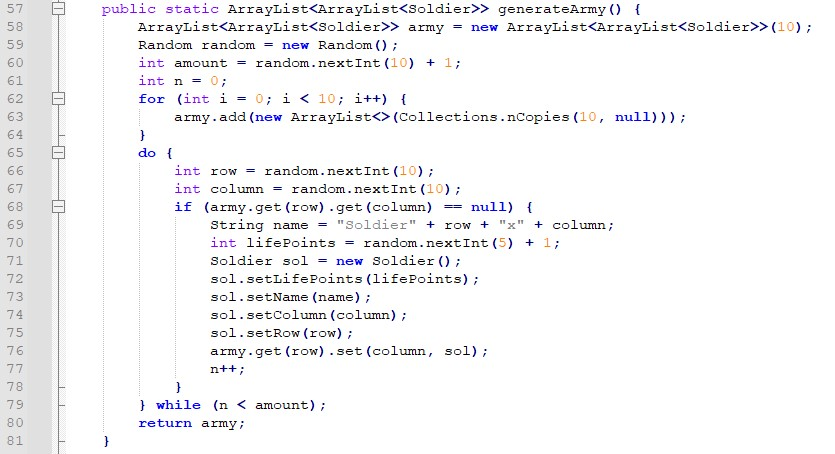
\includegraphics[width=1\textwidth,keepaspectratio]{img/1.jpg}
		%\includesvg{img/automata.svg}
		%\label{img:mot2}
		%\caption{Product backlog.}
	\end{figure}
	
	\begin{itemize}	
		\item El método generateArmy()  crea un arreglo bidimensional de 10 filas y 10 columnas con
		el fin de cubrir la misma cantidad de casillas del tablero, por
		lo que habrán posiciones que quedarán vacías ya que la cantidad de elementos del arreglo será un número aleatoria que oscila entre 1 a 10. También se genera el nombre de cada Soldier y
		sus puntos de vida de forma aleatoria. Este arreglo nos servirá más que nada para imprimir el
		tablero de una forma más sencilla.
		\item Como sabemos, el ArrayList es una estructura de datos compacta, es decir puede recibir n cantidad de elementos y esos elementos se acomodarán, por lo que no hay posiciones con elementos vacíos, pero es posible inicializar algunas posiciones con ningún elemento, en nuestro caso null, y eso hace el primer for, se encarga de llenar el ArrayList con null
	\end{itemize}
	
	
	\begin{lstlisting}[language=bash,caption={Commit: Metodo que genera un ejercito}][H]
		git add VideoJuego3.java
		git commit -m "Metodo que genera un ejercito"			
		git push -u origin main
	\end{lstlisting}
	
	\begin{lstlisting}[language=bash,caption={Se implementa el método que imprime el tablero con los soldados ya ubicados  }][H]
		notepad++ VideoJuego3.java
	\end{lstlisting}
	
		\begin{figure}[H]
		\centering
		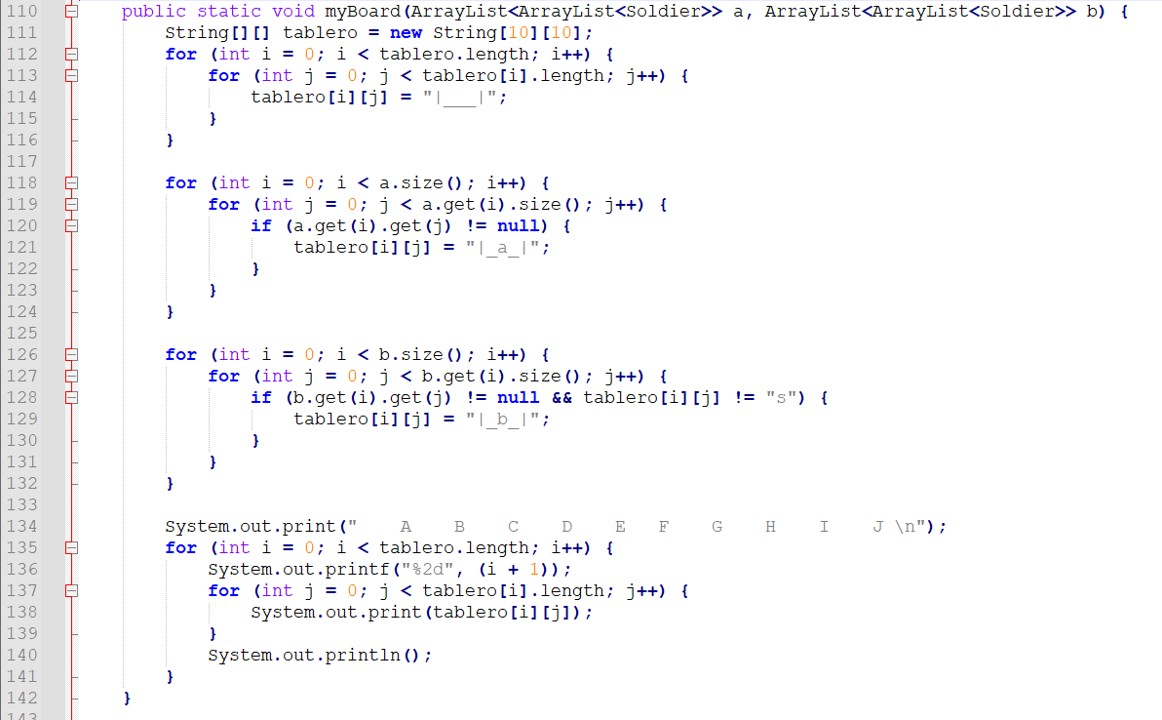
\includegraphics[width=1\textwidth,keepaspectratio]{img/2.jpg}
		%\includesvg{img/automata.svg}
		%\label{img:mot2}
		%\caption{Product backlog.}
	\end{figure}
	
	\begin{itemize}	
		\item Este método recibe como parámetros dos ArrayList bidimensionales de tipo Soldier. Se hace uso de 4 ciclos for. El primer for nos permite generar un arreglo bidimensional de caracteres que simularán el tablero. El segundo for se encarga de posicionar a los soldados del ejército A. El tercer for se encarga de posicionar a los soldados del ejército B. El último for se encarga imprimir el tablero con las posiciones y entradas correspondientes.
	\end{itemize}
		


	\begin{lstlisting}[language=bash,caption={Compilando y probando el tablero  }][H]
	javac VideoJuego3.java
	java VideoJuego3
	oooooooooooooooo  FASE 1 DE LA CONTIENDA  oooooooooooooooo
	Mostrando estadisticas de cada ejercito
	
	oooooooooooooooo  FASE 2 DE LA CONTIENDA  oooooooooooooooo
	Mostrando el tablero de juego
		A      B    C     D     E     F    G    H    I     J
	1 |___||___||___||___||___||___||___||___||___||___|
	2 |___||___||___||___||_b_||___||___||___||___||___|
	3 |___||___||___||___||_b_||___||___||___||___||___|
	4 |___||_b_||___||___||___||___||___||___||___||_a_|
	5 |___||___||___||___||___||___||___||___||___||___|
	6 |___||___||___||___||___||___||___||___||___||___|
	7 |___||___||___||___||___||___||___||___||___||___|
	8 |___||___||___||___||___||___||___||___||___||___|
	9 |___||___||___||_b_||___||___||___||___||___||___|
	10|___||___||___||___||___||___||___||___||___||___|
	\end{lstlisting}
	
	
	\begin{lstlisting}[language=bash,caption={Commit: Metodo que imprime el tablero completo}][H]
		git add VideoJuego3.java
		git commit -m "Metodo que imprime el tablero completo"			
		git push -u origin main
	\end{lstlisting}
	
	
	\begin{lstlisting}[language=bash,caption={Se implementa el método que genera un ArrayList unidimensional }][H]
		notepad++ VideoJuego3.java
	\end{lstlisting}
	
	\begin{figure}[H]
		\centering
		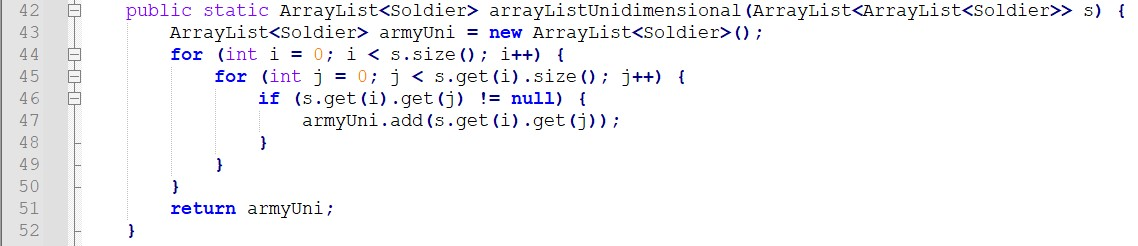
\includegraphics[width=1.1\textwidth,keepaspectratio]{img/3.jpg}
		%\includesvg{img/automata.svg}
		%\label{img:mot2}
		%\caption{Product backlog.}
	\end{figure}
	
	\begin{itemize}	
		\item A pesar de ya contar con dos ArrayList bidimensionales, se opta por transformarlos en ArrayList unidimensionales ya que nos facilitará trabajar con los demás métodos que la práctica de laboratorio solicita. En el main se hace la creación de dos ArrayList unidimensionales tanto para el ejército A y B.
	\end{itemize}
	
	
	\begin{lstlisting}[language=bash,caption={Commit: Metodo que convierte un ArrayList Bidimensional a Unidimensional}][H]
		git add VideoJuego3.java
		git commit -m "Metodo que convierte un ArrayList Bidimensional a Unidimensional"			
		git push -u origin main
	\end{lstlisting}
	
	
	
	
	
	
	\begin{lstlisting}[language=bash,caption={Se implementa el método que muestra los datos del ArrayList unidimensional según su orden de creación}][H]
		notepad++ VideoJuego3.java
	\end{lstlisting}
	
	\begin{figure}[H]
		\centering
		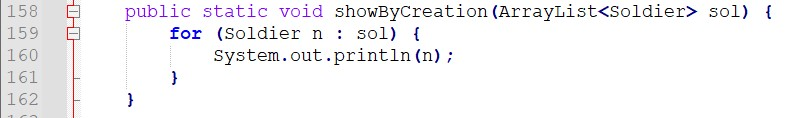
\includegraphics[width=1\textwidth,keepaspectratio]{img/4.jpg}
		%\includesvg{img/automata.svg}
		%\label{img:mot2}
		%\caption{Product backlog.}
	\end{figure}
	
	\begin{itemize}	
		\item Para tener una claridad de lo que se está haciendo, recién se decide implementar este método para ver si se está imprimiendo correctamente las posiciones de los soldados en el tablero.
	\end{itemize}
	
	\begin{lstlisting}[language=bash,caption={Compilando y probando}][H]
		javac VideoJuego3.java
		java VideoJuego3
		oooooooooooooooo  FASE 1 DE LA CONTIENDA  oooooooooooooooo
		Mostrando estadisticas de cada ejercito
		
		Mostrando soldados por orden de creacion
		DATOS DEL DEL EJERCITO A
		Soldier [name=Soldier0x6, lifePoints=3, row=1, column=7]
		Soldier [name=Soldier1x7, lifePoints=3, row=2, column=8]
		Soldier [name=Soldier3x6, lifePoints=4, row=4, column=7]
		Soldier [name=Soldier4x1, lifePoints=1, row=5, column=2]
		Soldier [name=Soldier4x2, lifePoints=1, row=5, column=3]
		Soldier [name=Soldier5x0, lifePoints=3, row=6, column=1]
		Soldier [name=Soldier5x3, lifePoints=3, row=6, column=4]
		Soldier [name=Soldier7x9, lifePoints=3, row=8, column=10]
		Soldier [name=Soldier8x4, lifePoints=5, row=9, column=5]
		
		DATOS DEL EJERCITO B
		Soldier [name=Soldier0x0, lifePoints=2, row=1, column=1]
		Soldier [name=Soldier8x5, lifePoints=1, row=9, column=6]
		Soldier [name=Soldier8x8, lifePoints=4, row=9, column=9]
		oooooooooooooooo  FASE 2 DE LA CONTIENDA  oooooooooooooooo
		Mostrando el tablero de juego
			A      B    C     D     E     F    G    H    I     J
		1 |_b_||___||___||___||___||___||_a_||___||___||___|
		2 |___||___||___||___||___||___||___||_a_||___||___|
		3 |___||___||___||___||___||___||___||___||___||___|
		4 |___||___||___||___||___||___||_a_||___||___||___|
		5 |___||_a_||_a_||___||___||___||___||___||___||___|
		6 |_a_||___||___||_a_||___||___||___||___||___||___|
		7 |___||___||___||___||___||___||___||___||___||___|
		8 |___||___||___||___||___||___||___||___||___||_a_|
		9 |___||___||___||___||_a_||_b_||___||___||_b_||___|
		10|___||___||___||___||___||___||___||___||___||___|
	\end{lstlisting}
	
	\begin{itemize}	
		\item Si observamos, nos damos cuenta que en el tablero falta generar la posición de un soldado del ejército B. Esto nos hace indicar que no se está haciendo correctamente el reemplazo para generar el tablero.
	\end{itemize}
	
		
	\begin{lstlisting}[language=bash,caption={Commit: Método que muestra los datos del ArrayList}][H]
		git add VideoJuego3.java
		git commit -m "Metodo que muestra los datos del ArrayList"			
		git push -u origin main
	\end{lstlisting}
	
	
	
	\begin{lstlisting}[language=bash,caption={Se implementa un método que genera un ArrayList para el ejército B}][H]
		notepad++ VideoJuego3.java
	\end{lstlisting}
	
	\begin{figure}[H]
		\centering
		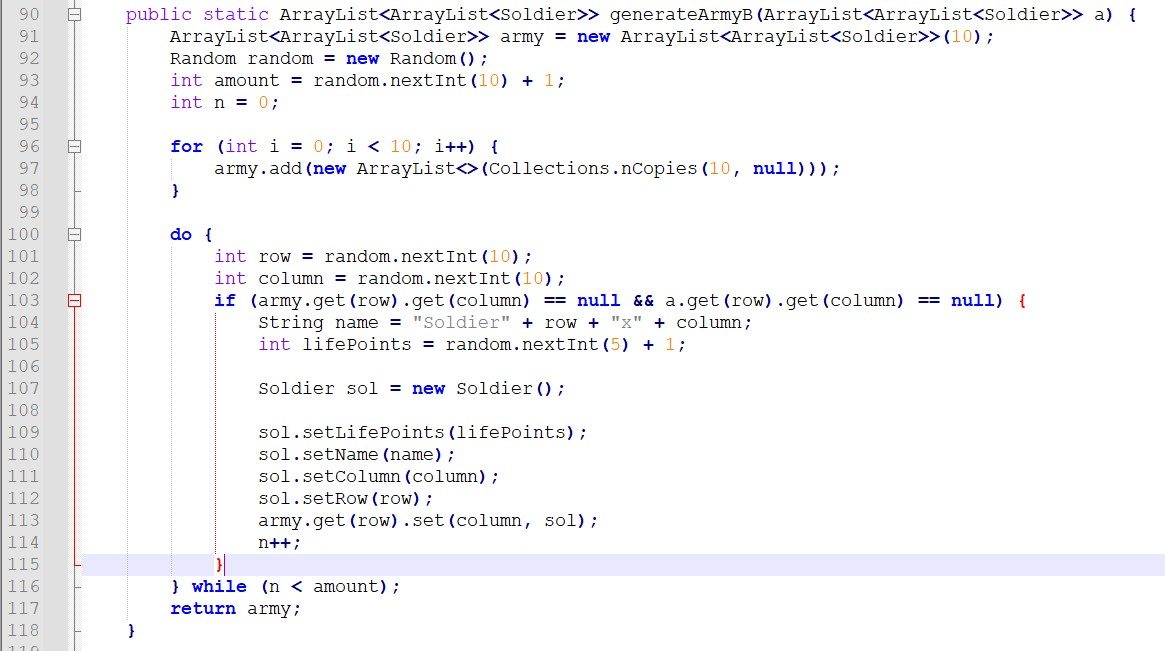
\includegraphics[width=1.1\textwidth,keepaspectratio]{img/5.jpg}
		%\includesvg{img/automata.svg}
		%\label{img:mot2}
		%\caption{Product backlog.}
	\end{figure}
	
	\begin{itemize}	
		\item La razón de la creación de este método se debe a que hay casos en los que la cantidad de fichas del ejército B que están ubicadas en el tablero no coincide en cantidad con lo que se genera, eso se comprobó cuando se decidió compilar el método showByCreation.
		\item Básicamente este método es igual que generateArmy, solo que este método recibe un parámetro de tipo ArrayList Bidimensional- Soldier que se usará para verificar que se generen los soldados del ejército B sin que haya cruces con los del ejército A, por lo que en la estructura condicional se añade esta línea a.get(row).get(column) == null 
	\end{itemize}
	
	\begin{lstlisting}[language=bash,caption={Compilando y probando las correcciones}][H]
		javac VideoJuego3.java
		java VideoJuego3
		oooooooooooooooo  FASE 1 DE LA CONTIENDA  oooooooooooooooo
		Mostrando estadisticas de cada ejercito
		
		Mostrando soldados por orden de creacion
		DATOS DEL DEL EJERCITO A
		Soldier [name=Soldier6x6, lifePoints=1, row=7, column=7]
		
		DATOS DEL EJERCITO B
		Soldier [name=Soldier3x5, lifePoints=3, row=4, column=6]
		Soldier [name=Soldier5x8, lifePoints=1, row=6, column=9]
		Soldier [name=Soldier8x1, lifePoints=1, row=9, column=2]
		Soldier [name=Soldier9x6, lifePoints=5, row=10, column=7]
		oooooooooooooooo  FASE 2 DE LA CONTIENDA  oooooooooooooooo
		Mostrando el tablero de juego
	 		A      B    C     D     E     F    G    H    I     J
		1 |___||___||___||___||___||___||___||___||___||___|
		2 |___||___||___||___||___||___||___||___||___||___|
		3 |___||___||___||___||___||___||___||___||___||___|
		4 |___||___||___||___||___||_b_||___||___||___||___|
		5 |___||___||___||___||___||___||___||___||___||___|
		6 |___||___||___||___||___||___||___||___||_b_||___|
		7 |___||___||___||___||___||___||_a_||___||___||___|
		8 |___||___||___||___||___||___||___||___||___||___|
		9 |___||_b_||___||___||___||___||___||___||___||___|
		10|___||___||___||___||___||___||_b_||___||___||___|
	\end{lstlisting}
	\begin{itemize}	
		\item Para aclarar, en el main se corrigió la forma en la que se crea el ArrayList para el ejército B
	\end{itemize}

	\begin{lstlisting}[language=bash,caption={Commit: Metodo que genera un arreglo bidimensional para el ejercito B}][H]
		git add VideoJuego3.java
		git commit -m "Metodo que genera un arreglo bidimensional para el ejercito B"			
		git push -u origin main
	\end{lstlisting}
	
	
	
	
	
	
	\begin{lstlisting}[language=bash,caption={Se implementa el método que busca al soldado con mayor puntaje de vida}][H]
		notepad++ VideoJuego3.java
	\end{lstlisting}
	
	\begin{figure}[H]
		\centering
		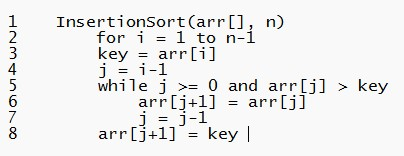
\includegraphics[width=1\textwidth,keepaspectratio]{img/insertion.jpg}
		%\includesvg{img/automata.svg}
		%\label{img:mot2}
		%\caption{Product backlog.}
	\end{figure}
	
		
	\begin{itemize}	
		\item Se hace uso del método de ordenamiento Insertion.
	\end{itemize}
	
	\begin{figure}[H]
		\centering
		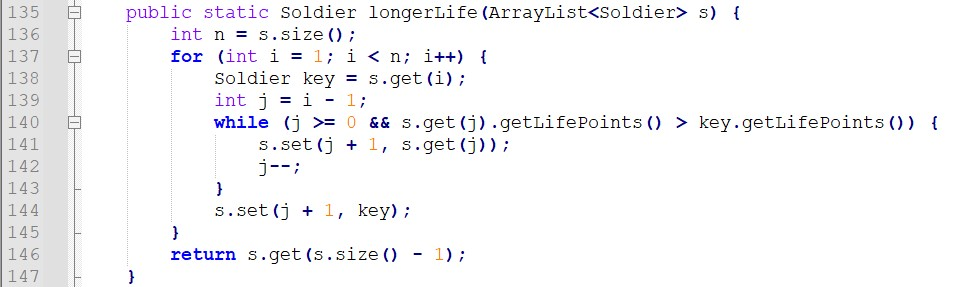
\includegraphics[width=1\textwidth,keepaspectratio]{img/6.jpg}
		%\includesvg{img/automata.svg}
		%\label{img:mot2}
		%\caption{Product backlog.}
	\end{figure}
	
	\begin{itemize}	
		\item Lo que hace el método es ordenar de menor a mayor, por lo que último elemento es el mayor. El método devuelve al Soldier que se encuentra en esa posición.
	\end{itemize}
	
	
	\begin{lstlisting}[language=bash,caption={Compilando y probando }][H]
		javac VideoJuego3.java
		java VideoJuego3
		oooooooooooooooo  FASE 1 DE LA CONTIENDA  oooooooooooooooo
		Mostrando estadisticas de cada ejercito
		
		Mostrando soldados por orden de creacion
		DATOS DEL DEL EJERCITO A
		Soldier [name=Soldier0x1, lifePoints=2, row=1, column=2]
		Soldier [name=Soldier2x5, lifePoints=3, row=3, column=6]
		Soldier [name=Soldier6x3, lifePoints=2, row=7, column=4]
		Soldier [name=Soldier7x4, lifePoints=1, row=8, column=5]
		Soldier [name=Soldier8x8, lifePoints=5, row=9, column=9]
		Soldier [name=Soldier9x5, lifePoints=3, row=10, column=6]
		Mayor vida en A: Soldier [name=Soldier8x8, lifePoints=5, row=9, column=9]
		
		DATOS DEL EJRCITO B
		Soldier [name=Soldier1x0, lifePoints=2, row=2, column=1]
		Soldier [name=Soldier5x1, lifePoints=5, row=6, column=2]
		Soldier [name=Soldier6x6, lifePoints=4, row=7, column=7]
		Soldier [name=Soldier8x0, lifePoints=2, row=9, column=1]
		Mayor vida en B: Soldier [name=Soldier5x1, lifePoints=5, row=6, column=2]
		oooooooooooooooo  FASE 2 DE LA CONTIENDA  oooooooooooooooo
		Mostrando el tablero de juego
			A      B    C     D     E     F    G    H    I     J
		1 |___||_a_||___||___||___||___||___||___||___||___|
		2 |_b_||___||___||___||___||___||___||___||___||___|
		3 |___||___||___||___||___||_a_||___||___||___||___|
		4 |___||___||___||___||___||___||___||___||___||___|
		5 |___||___||___||___||___||___||___||___||___||___|
		6 |___||_b_||___||___||___||___||___||___||___||___|
		7 |___||___||___||_a_||___||___||_b_||___||___||___|
		8 |___||___||___||___||_a_||___||___||___||___||___|
		9 |_b_||___||___||___||___||___||___||___||_a_||___|
		10|___||___||___||___||___||_a_||___||___||___||___|
	\end{lstlisting}
	
	\begin{lstlisting}[language=bash,caption={Commit: Metodo longerLife culminado B}][H]
		git add VideoJuego3.java
		git commit -m "Metodo longerLife culminado"			
		git push -u origin main
	\end{lstlisting}
	
	
	\begin{lstlisting}[language=bash,caption={Se implementa el método que retorna la vida total del ejército}][H]
		notepad++ VideoJuego3.java
	\end{lstlisting}
	
	\begin{figure}[H]
		\centering
		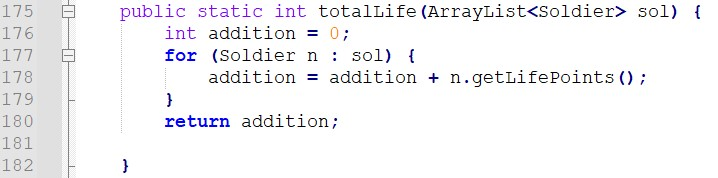
\includegraphics[width=1\textwidth,keepaspectratio]{img/7.jpg}
		%\includesvg{img/automata.svg}
		%\label{img:mot2}
		%\caption{Product backlog.}
	\end{figure}
	
	
	\begin{itemize}	
		\item El método devuelve los puntos de vida total del ejército. Se decide hacer el método con retorno para poder usar esos valores en otro método que nos permitirá determinar al ganador.
	\end{itemize}
	
	\begin{lstlisting}[language=bash,caption={Commit: Metodo totalLife culminado B}][H]
		git add VideoJuego3.java
		git commit -m "Metodo totalLife culminado"			
		git push -u origin main
	\end{lstlisting}	
	
	
	
	\begin{lstlisting}[language=bash,caption={Se implementa el código que calculará el promedio de vida de cada ejército}][H]
		notepad++ VideoJuego3.java
	\end{lstlisting}
	
	\begin{figure}[H]
		\centering
		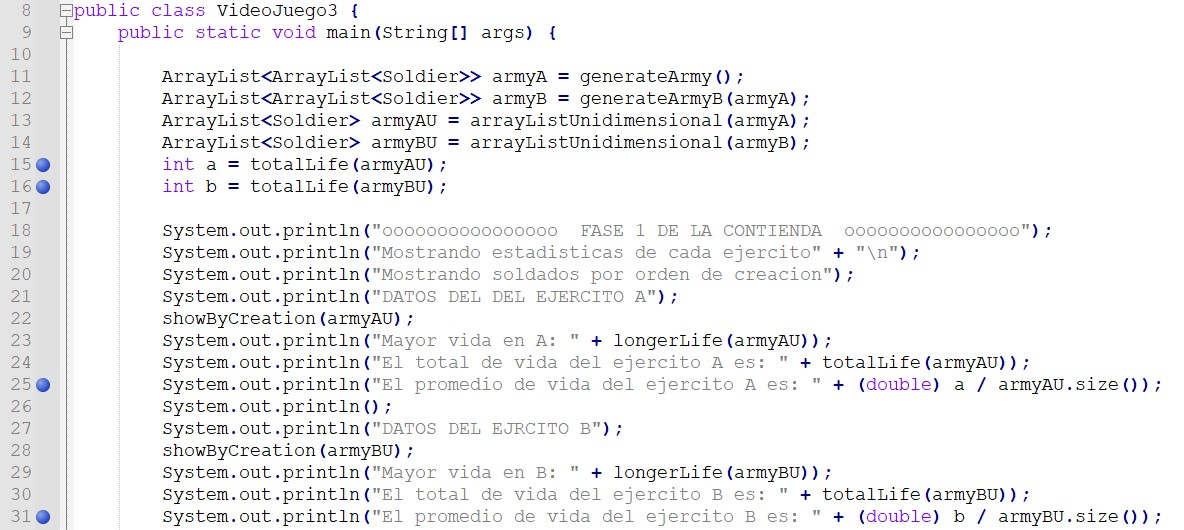
\includegraphics[width=1.1\textwidth,keepaspectratio]{img/8.jpg}
		%\includesvg{img/automata.svg}
		%\label{img:mot2}
		%\caption{Product backlog.}
	\end{figure}
	
	
	\begin{itemize}	
		\item Lo que está en azul, al costado de los números, es la implementación del código para calcular el promedio.
	\end{itemize}
	
	
	\begin{lstlisting}[language=bash,caption={Compilando y probando }][H]
		javac VideoJuego3.java
		java VideoJuego3
		oooooooooooooooo  FASE 1 DE LA CONTIENDA  oooooooooooooooo
		Mostrando estadisticas de cada ejercito
		
		Mostrando soldados por orden de creacion
		DATOS DEL DEL EJERCITO A
		Soldier [name=Soldier0x1, lifePoints=3, row=1, column=2]
		Soldier [name=Soldier1x4, lifePoints=4, row=2, column=5]
		Soldier [name=Soldier7x4, lifePoints=2, row=8, column=5]
		Mayor vida en A: Soldier [name=Soldier1x4, lifePoints=4, row=2, column=5]
		El total de vida del ejercito A es: 9
		El promedio de vida del ejercito A es: 3.0
		
		DATOS DEL EJRCITO B
		Soldier [name=Soldier4x4, lifePoints=1, row=5, column=5]
		Soldier [name=Soldier7x5, lifePoints=4, row=8, column=6]
		Soldier [name=Soldier9x8, lifePoints=5, row=10, column=9]
		Mayor vida en B: Soldier [name=Soldier9x8, lifePoints=5, row=10, column=9]
		El total de vida del ejercito B es: 10
		El promedio de vida del ejercito B es: 3.3333333333333335
		oooooooooooooooo  FASE 2 DE LA CONTIENDA  oooooooooooooooo
		Mostrando el tablero de juego
		    A      B    C     D     E     F    G    H    I     J
		1 |___||_a_||___||___||___||___||___||___||___||___|
		2 |___||___||___||___||_a_||___||___||___||___||___|
		3 |___||___||___||___||___||___||___||___||___||___|
		4 |___||___||___||___||___||___||___||___||___||___|
		5 |___||___||___||___||_b_||___||___||___||___||___|
		6 |___||___||___||___||___||___||___||___||___||___|
		7 |___||___||___||___||___||___||___||___||___||___|
		8 |___||___||___||___||_a_||_b_||___||___||___||___|
		9 |___||___||___||___||___||___||___||___||___||___|
		10|___||___||___||___||___||___||___||___||_b_||___|
	\end{lstlisting}
	
	
	\begin{lstlisting}[language=bash,caption={Commit:Codigo para calcular el promedio de vida para cada ejercito}][H]
		git add VideoJuego3.java
		git commit -m "Codigo para calcular el promedio de vida para cada ejercito"			
		git push -u origin main
	\end{lstlisting}	
	
	
	
	
	\begin{lstlisting}[language=bash,caption={Se implementa el método que ordena el ArrayList mostrando un ranking}][H]
		notepad++ VideoJuego3.java
	\end{lstlisting}
	
	\begin{figure}[H]
		\centering
		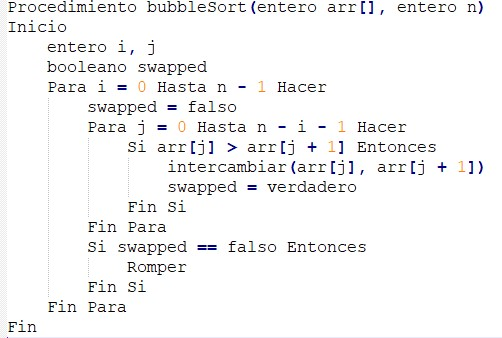
\includegraphics[width=0.9\textwidth,keepaspectratio]{img/burbuja.jpg}
		%\includesvg{img/automata.svg}
		%\label{img:mot2}
		%\caption{Product backlog.}
	\end{figure}
	
	
	\begin{itemize}	
		\item Para este método se hará uso del método de ordenamiento Burbuja
	\end{itemize}
	
	
	\begin{figure}[H]
		\centering
		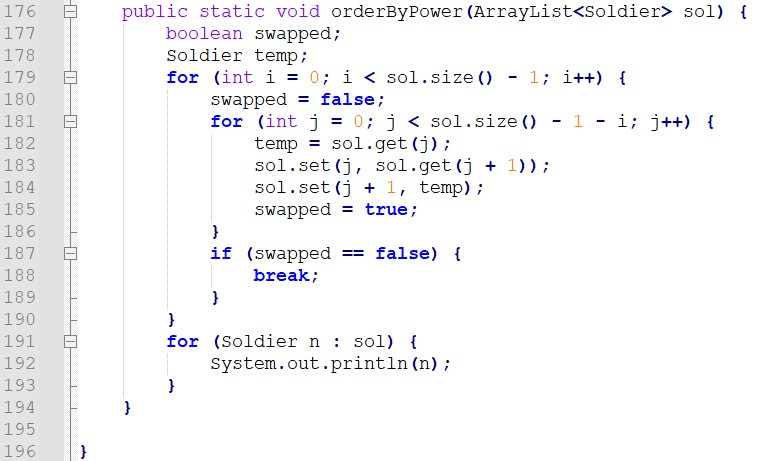
\includegraphics[width=1.1\textwidth,keepaspectratio]{img/9.jpg}
		%\includesvg{img/automata.svg}
		%\label{img:mot2}
		%\caption{Product backlog.}
	\end{figure}
	
	
	\begin{itemize}	
		\item El método ordena el ArrayList y se imprime el ranking, por lo que no retorna nada
	\end{itemize}
	
	
	\begin{lstlisting}[language=bash,caption={Compilando y probando }][H]
		javac VideoJuego3.java
		java VideoJuego3
		oooooooooooooooo  FASE 1 DE LA CONTIENDA  oooooooooooooooo
		Mostrando estadisticas de cada ejercito
		
		Mostrando soldados por orden de creacion
		DATOS DEL DEL EJERCITO A
		Soldier [name=Soldier0x7, lifePoints=5, row=1, column=8]
		Soldier [name=Soldier1x1, lifePoints=5, row=2, column=2]
		Soldier [name=Soldier4x9, lifePoints=1, row=5, column=10]
		Soldier [name=Soldier5x7, lifePoints=2, row=6, column=8]
		Soldier [name=Soldier8x9, lifePoints=3, row=9, column=10]
		Mayor vida en A: Soldier [name=Soldier1x1, lifePoints=5, row=2, column=2]
		El total de vida del ejercito A es: 16
		El promedio de vida del ejercito A es: 3.2
		Mostrando soldados por ranking de poder de A
		Soldier [name=Soldier1x1, lifePoints=5, row=2, column=2]
		Soldier [name=Soldier0x7, lifePoints=5, row=1, column=8]
		Soldier [name=Soldier8x9, lifePoints=3, row=9, column=10]
		Soldier [name=Soldier5x7, lifePoints=2, row=6, column=8]
		Soldier [name=Soldier4x9, lifePoints=1, row=5, column=10]
		
		DATOS DEL EJRCITO B
		Soldier [name=Soldier3x4, lifePoints=1, row=4, column=5]
		Soldier [name=Soldier5x9, lifePoints=4, row=6, column=10]
		Soldier [name=Soldier7x6, lifePoints=1, row=8, column=7]
		Soldier [name=Soldier7x8, lifePoints=5, row=8, column=9]
		Soldier [name=Soldier9x9, lifePoints=4, row=10, column=10]
		Mayor vida en B: Soldier [name=Soldier7x8, lifePoints=5, row=8, column=9]
		El total de vida del ejercito B es: 15
		El promedio de vida del ejercito B es: 3.0
		Mostrando soldados por ranking de poder de B
		Soldier [name=Soldier7x8, lifePoints=5, row=8, column=9]
		Soldier [name=Soldier9x9, lifePoints=4, row=10, column=10]
		Soldier [name=Soldier5x9, lifePoints=4, row=6, column=10]
		Soldier [name=Soldier7x6, lifePoints=1, row=8, column=7]
		Soldier [name=Soldier3x4, lifePoints=1, row=4, column=5]
		oooooooooooooooo  FASE 2 DE LA CONTIENDA  oooooooooooooooo
		Mostrando el tablero de juego
		    A      B    C     D     E     F    G    H    I     J
		1 |___||___||___||___||___||___||___||_a_||___||___|
		2 |___||_a_||___||___||___||___||___||___||___||___|
		3 |___||___||___||___||___||___||___||___||___||___|
		4 |___||___||___||___||_b_||___||___||___||___||___|
		5 |___||___||___||___||___||___||___||___||___||_a_|
		6 |___||___||___||___||___||___||___||_a_||___||_b_|
		7 |___||___||___||___||___||___||___||___||___||___|
		8 |___||___||___||___||___||___||_b_||___||_b_||___|
		9 |___||___||___||___||___||___||___||___||___||_a_|
		10|___||___||___||___||___||___||___||___||___||_b_|
	\end{lstlisting}
	
	
	
	\begin{lstlisting}[language=bash,caption={Commit:Se ha implementado el metodo orderByPower en el main}][H]
		git add VideoJuego3.java
		git commit -m "Se ha implementado el metodo orderByPower en el main"			
		git push -u origin main
	\end{lstlisting}
	
	
	
	
	
	\begin{lstlisting}[language=bash,caption={Se implementa el método que determina al ganador}][H]
		notepad++ VideoJuego3.java
	\end{lstlisting}
	
	\begin{figure}[H]
		\centering
		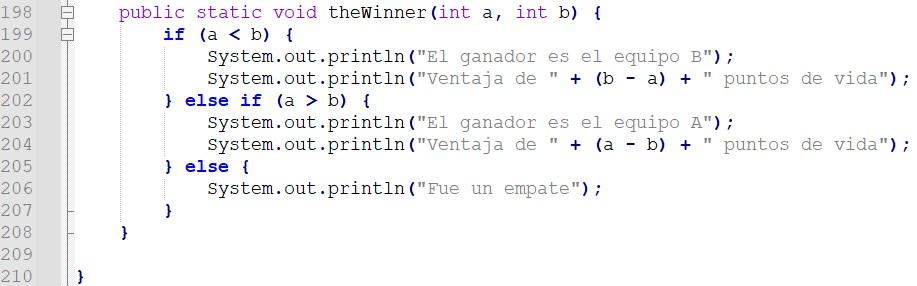
\includegraphics[width=1.1\textwidth,keepaspectratio]{img/10.jpg}
		%\includesvg{img/automata.svg}
		%\label{img:mot2}
		%\caption{Product backlog.}
	\end{figure}
	
	
	\begin{itemize}	
		\item Para determinar a un ganador, se opta por enfrentarlos de acuerdo a su cantidad de puntos de vida.
	\end{itemize}
	
	
	\begin{figure}[H]
		\centering
		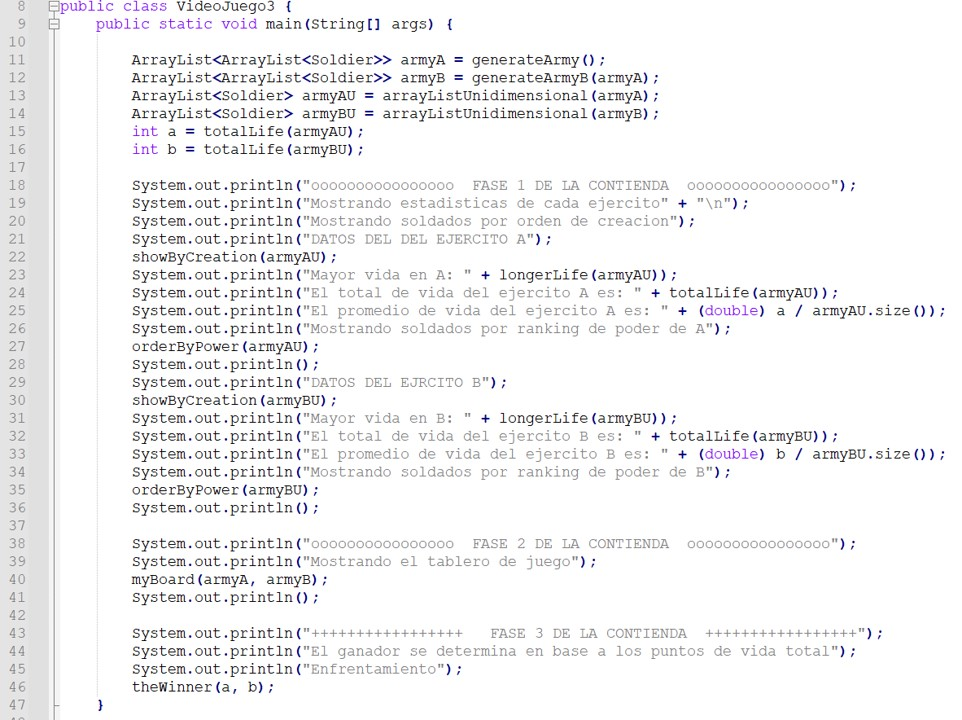
\includegraphics[width=1.1\textwidth,keepaspectratio]{img/main.jpg}
		%\includesvg{img/automata.svg}
		%\label{img:mot2}
		%\caption{Product backlog.}
	\end{figure}
	
	\begin{itemize}	
		\item En esta parte del código se tiene al Main el cual contiene la llamada de los métodos. Finalmente así quedaría el código.
	\end{itemize}
	
	
	\begin{lstlisting}[language=bash,caption={Compilando y probando el codigo en su versión final }][H]
		javac VideoJuego3.java
		java VideoJuego3
		oooooooooooooooo  FASE 1 DE LA CONTIENDA  oooooooooooooooo
		Mostrando estadisticas de cada ejercito
		
		Mostrando soldados por orden de creacion
		DATOS DEL DEL EJERCITO A
		Soldier [name=Soldier0x2, lifePoints=5, row=1, column=3]
		Soldier [name=Soldier0x4, lifePoints=3, row=1, column=5]
		Soldier [name=Soldier1x0, lifePoints=1, row=2, column=1]
		Soldier [name=Soldier2x2, lifePoints=3, row=3, column=3]
		Soldier [name=Soldier4x6, lifePoints=3, row=5, column=7]
		Soldier [name=Soldier4x9, lifePoints=3, row=5, column=10]
		Soldier [name=Soldier6x2, lifePoints=2, row=7, column=3]
		Soldier [name=Soldier8x9, lifePoints=3, row=9, column=10]
		Soldier [name=Soldier9x2, lifePoints=5, row=10, column=3]
		Mayor vida en A: Soldier [name=Soldier9x2, lifePoints=5, row=10, column=3]
		El total de vida del ejercito A es: 28
		El promedio de vida del ejercito A es: 3.111111111111111
		Mostrando soldados por ranking de poder de A
		Soldier [name=Soldier9x2, lifePoints=5, row=10, column=3]
		Soldier [name=Soldier0x2, lifePoints=5, row=1, column=3]
		Soldier [name=Soldier8x9, lifePoints=3, row=9, column=10]
		Soldier [name=Soldier4x9, lifePoints=3, row=5, column=10]
		Soldier [name=Soldier4x6, lifePoints=3, row=5, column=7]
		Soldier [name=Soldier2x2, lifePoints=3, row=3, column=3]
		Soldier [name=Soldier0x4, lifePoints=3, row=1, column=5]
		Soldier [name=Soldier6x2, lifePoints=2, row=7, column=3]
		Soldier [name=Soldier1x0, lifePoints=1, row=2, column=1]
		
		DATOS DEL EJRCITO B
		Soldier [name=Soldier0x3, lifePoints=4, row=1, column=4]
		Soldier [name=Soldier0x7, lifePoints=1, row=1, column=8]
		Soldier [name=Soldier1x1, lifePoints=2, row=2, column=2]
		Soldier [name=Soldier4x3, lifePoints=4, row=5, column=4]
		Soldier [name=Soldier6x6, lifePoints=5, row=7, column=7]
		Soldier [name=Soldier9x9, lifePoints=2, row=10, column=10]
		Mayor vida en B: Soldier [name=Soldier6x6, lifePoints=5, row=7, column=7]
		El total de vida del ejercito B es: 18
		El promedio de vida del ejercito B es: 3.0
		Mostrando soldados por ranking de poder de B
		Soldier [name=Soldier6x6, lifePoints=5, row=7, column=7]
		Soldier [name=Soldier4x3, lifePoints=4, row=5, column=4]
		Soldier [name=Soldier0x3, lifePoints=4, row=1, column=4]
		Soldier [name=Soldier9x9, lifePoints=2, row=10, column=10]
		Soldier [name=Soldier1x1, lifePoints=2, row=2, column=2]
		Soldier [name=Soldier0x7, lifePoints=1, row=1, column=8]
		
		oooooooooooooooo  FASE 2 DE LA CONTIENDA  oooooooooooooooo
		Mostrando el tablero de juego
			A      B    C     D     E     F    G    H    I     J
		1 |___||___||_a_||_b_||_a_||___||___||_b_||___||___|
		2 |_a_||_b_||___||___||___||___||___||___||___||___|
		3 |___||___||_a_||___||___||___||___||___||___||___|
		4 |___||___||___||___||___||___||___||___||___||___|
		5 |___||___||___||_b_||___||___||_a_||___||___||_a_|
		6 |___||___||___||___||___||___||___||___||___||___|
		7 |___||___||_a_||___||___||___||_b_||___||___||___|
		8 |___||___||___||___||___||___||___||___||___||___|
		9 |___||___||___||___||___||___||___||___||___||_a_|
		10|___||___||_a_||___||___||___||___||___||___||_b_|
		
		+++++++++++++++++   FASE 3 DE LA CONTIENDA  +++++++++++++++++
		El ganador se determina en base a los puntos de vida total
		Enfrentamiento
		El ganador es el equipo A
		Ventaja de 10 puntos de vida
	\end{lstlisting}
	
	
	\begin{lstlisting}[language=bash,caption={Commit:Se ha aumentado codigo en el main y el metodo theWinner}][H]
		git add VideoJuego3.java
		git commit -m "Se ha aumentado codigo en el main y el metodo theWinner"			
		git push -u origin main
	\end{lstlisting}
	
	

	
	\subsection{Estructura de laboratorio 06}
	\begin{itemize}	
		\item El contenido que se entrega en este laboratorio es el siguiente:
	\end{itemize}
	
	\begin{lstlisting}[style=ascii-tree]
		lab06
		|- -Soldier.java
		|- -VideoJuego3.java
		|
		 ─ ─latex
			|   programacion_lab06_rescobedoq_v1.0.pdf
			|   programacion_lab06_rescobedoq_v1.0.tex
			|
			 ─ ─img
					1.jpg
					10.jpg
					2.jpg
					3.jpg
					4.jpg
					5.jpg
					6.jpg
					7.jpg
					8.jpg
					9.jpg
					burbuja.jpg
					insertion.jpg
					logo_abet.png
					logo_episunsa.png
					logo_unsa.jpg
					main.jpg
		
		
	\end{lstlisting}    
	
	\section{\textcolor{red}{Rúbricas}}
	
	\subsection{\textcolor{red}{Entregable Informe}}
	\begin{table}[H]
		\caption{Tipo de Informe}
		\setlength{\tabcolsep}{0.5em} % for the horizontal padding
		{\renewcommand{\arraystretch}{1.5}% for the vertical padding
			\begin{tabular}{|p{3cm}|p{12cm}|}
				\hline
				\multicolumn{2}{|c|}{\textbf{\textcolor{red}{Informe}}}  \\
				\hline 
				\textbf{\textcolor{red}{Latex}} & \textcolor{blue}{El informe está en formato PDF desde Latex,  con un formato limpio (buena presentación) y facil de leer.}   \\ 
				\hline 
				
				
			\end{tabular}
		}
	\end{table}
	
	\clearpage
	
	\subsection{\textcolor{red}{Rúbrica para el contenido del Informe y demostración}}
	\begin{itemize}			
		\item El alumno debe marcar o dejar en blanco en celdas de la columna \textbf{Checklist} si cumplio con el ítem correspondiente.
		\item Si un alumno supera la fecha de entrega,  su calificación será sobre la nota mínima aprobada, siempre y cuando cumpla con todos lo items.
		\item El alumno debe autocalificarse en la columna \textbf{Estudiante} de acuerdo a la siguiente tabla:
		
		\begin{table}[ht]
			\caption{Niveles de desempeño}
			\begin{center}
				\begin{tabular}{ccccc}
					\hline
					& \multicolumn{4}{c}{Nivel}\\
					\cline{1-5}
					\textbf{Puntos} & Insatisfactorio 25\%& En Proceso 50\% & Satisfactorio 75\% & Sobresaliente 100\%\\
					\textbf{2.0}&0.5&1.0&1.5&2.0\\
					\textbf{4.0}&1.0&2.0&3.0&4.0\\
					\hline
				\end{tabular}
			\end{center}
		\end{table}	
		
	\end{itemize}
	
	\begin{table}[H]
		\caption{Rúbrica para contenido del Informe y demostración}
		\setlength{\tabcolsep}{0.5em} % for the horizontal padding
		{\renewcommand{\arraystretch}{1.5}% for the vertical padding
			%\begin{center}
			\begin{tabular}{|p{2.7cm}|p{7cm}|x{1.3cm}|p{1.2cm}|p{1.5cm}|p{1.1cm}|}
				\hline
				\multicolumn{2}{|c|}{Contenido y demostración} & Puntos & Checklist & Estudiante & Profesor\\
				\hline
				\textbf{1. GitHub} & Hay enlace URL activo del directorio para el  laboratorio hacia su repositorio GitHub con código fuente terminado y fácil de revisar. &2 &X &2 & \\ 
				\hline
				\textbf{2. Commits} &  Hay capturas de pantalla de los commits más importantes con sus explicaciones detalladas. (El profesor puede preguntar para refrendar calificación). &4 &X &4 & \\ 
				\hline 
				\textbf{3. Código fuente} &  Hay porciones de código fuente importantes con numeración y explicaciones detalladas de sus funciones. &2 &X &2 & \\ 
				\hline 
				\textbf{4. Ejecución} & Se incluyen ejecuciones/pruebas del código fuente  explicadas gradualmente. &2 &X &2 & \\ 
				\hline			
				\textbf{5. Pregunta} & Se responde con completitud a la pregunta formulada en la tarea.  (El profesor puede preguntar para refrendar calificación).  &2 &X &2 & \\ 
				\hline	
				\textbf{6. Fechas} & Las fechas de modificación del código fuente estan dentro de los plazos de fecha de entrega establecidos. &2 &X &2 & \\ 
				\hline 
				\textbf{7. Ortografía} & El documento no muestra errores ortográficos. &2 &X &1 & \\ 
				\hline 
				\textbf{8. Madurez} & El Informe muestra de manera general una evolución de la madurez del código fuente,  explicaciones puntuales pero precisas y un acabado impecable.   (El profesor puede preguntar para refrendar calificación).  &4 &X &3 & \\ 
				\hline
				\multicolumn{2}{|c|}{\textbf{Total}} &20 & &18 & \\ 
				\hline
			\end{tabular}
			%\end{center}
			%\label{tab:multicol}
		}
	\end{table}
	
	\clearpage
	
	\section{Referencias}
	\begin{itemize}			
		\item \url{https://www.geeksforgeeks.org/bubble-sort/}
		\item \url{https://www.geeksforgeeks.org/insertion-sort/}
	\end{itemize}	
	
	%\clearpage
	%\bibliographystyle{apalike}
	%\bibliographystyle{IEEEtranN}
	%\bibliography{bibliography}
	
\end{document}